% INPUT FILE FOR NUCLEAR ENGINEERING FACULTY
% ------------------------------------------------------------ 
% Each faculty member gets a faculty tile. (Formatting for this tile is defined in the preamble.)
% Each faculty tile is then included in a row of two tiles. (Its formatting also defined in the preamble.)
% The sytax is as follows:
% \facultyrow{
%		\facultytile{image_name_faculty1}
%		{Name faculty 1}
%		{Position faculty 1}
%		{Email faculty 1}
%		{Description faculty1}
%	}{
%		\facultytile{image_name_faculty2}
%		{Name faculty 2}
%		{Position faculty 2}
%		{Email faculty 2}
%		{Description faculty2}
%}
\newgeometry{margin=2cm,top=1.5cm}
\addcontentsline{toc}{section}{Faculty}
\section*{Faculty}
\vspace{0.5cm}

\facultyrow{
\facultytile{faculty/rebecca_abergel}
{Rebecca Abergel}
{Assistant Professor}
{abergel@berkeley.edu}
{Heavy element coordination and biological chemistry; fission product/transuranics/ medical isotopes separation, metabolism, and toxicity; drug development for radionuclide decontamination and radiotherapy.}
}{
\facultytile{faculty/lee_bernstein}
{Lee Bernstein}
{Adjunct Professor}
{labernstein@berkeley.edu}
{Statistical properties of nuclear matter; nuclear physics in high energy density plasmas; neutron-induced reaction cross section measurements; surrogate nuclear reactions.}
}
\facultyrow{
\facultytile{faculty/max_fratoni}
{Max Fratoni}
{Associate Professor}
{maxfratoni@berkeley.edu}
{Nuclear reactor theory, design and analysis, computation, and fuel cycle analysis. 
Focus resides on advanced fuels for generation IV reactors and designs for future reactors.}
}{
\facultytile{faculty/ehud_greenspan}
{Ehud Greenspan}
{Professor of the Graduate School}
{gehud@nuc.berkeley.edu}{Nuclear reactor theory, design and analysis. 
Conception, design and analysis of advanced (primarily, Generation-IV) nuclear reactors and advanced nuclear fuel cycles.}
}
\facultyrow{
\facultytile{faculty/peter_hosemann}
{Peter Hosemann}
{Associate Professor and Chair}
{peterh@berkeley.edu}
{Experimental material science for nuclear applications, mainly structural materials used for nuclear components (fission, fusion, spallation, etc.). 
Materials degradation processes in a nuclear environment and resulting consequences to engineering application.}
}{
\facultytile{faculty/daniel_kammen}
{Daniel M. Kammen}
{Professor of Energy}
{kammen@berkeley.edu}
{Science and technology policy focused on energy, development and environmental management. 
Technology and policy questions in developing nations. 
Global environmental change including deep cuts in greenhouse gas emissions and resource consumption. 
Management of innovation and energy R\&D policy.}
}
\facultyrow{
\facultytile{faculty/william_kastenberg}
{William Kastenberg}
{Professor Emeritus}
{}
{Ethical issues in emerging technologies, risk assessment and risk management for technological and natural complex systems, nuclear reactor safety, environmental risk analysis, environmental conflict resolution.}
}{
\facultytile{faculty/ka-ngo_leung}
{Ka-Ngo Leung}
{Professor-in-Residence}
{knleung@lbl.gov}
{Ion sources and their application. 
He has been awarded over 20 patents for the inventions of the ion sources and beam technologies for numerous applications.}
}
\facultyrow{
\facultytile{faculty/digby_macdonald}
{Digby Macdonald}
{Professor-in-Residence}
{macdonald@berkeley.edu}
{Aqueous corrosion and its prevention with special attention towards nuclear systems. 
Aqueous corrosion in extreme environments including high strength localized radiation fields and supercritical systems.}
}{
\facultytile{faculty/edward_morse}
{Edward C. Morse}
{Professor}
{morse@nuc.berkeley.edu}
{Fusion reactor design and applied plasma physics, experimental investigation of RF plasma heating. 
Rotating Target Neutron Source at UC Berkeley. 
Experimental Studies of Compact Toroids. 
A Spectral Method for Magnetohydrodynamic Stability}
}
\facultyrow{
\facultytile{faculty/eric_norman}
{Eric B. Norman}
{Professor of the Graduate School}
{ebnorman@lbl.gov}
{Nuclear physics for homeland security, neutrino physics, and nuclear astrophysics.}
}{
\facultytile{faculty/per_peterson}
{Per Peterson}
{Professor}
{peterson@nuc.berkeley.edu}
{High-temperature fission energy systems, and topics related to the safety and security of nuclear materials and waste management. 
His research group focuses primarily on heat transfer, fluid mechanics, regulation and licensing for high temperature reactors that use liquid fluoride salts as coolant.}
}
\facultyrow{
\facultytile{faculty/raluca_scarlat}
{Raluca O. Scarlat}
{Assistant Professor}
{scarlat@berkeley.edu}
{Chemical and termophysical characterization of high-temperature molten salts and other inorganic fluids, and heat and mass transport pertaining to energy systems; electrochemistry, corrosion, thermodynamics; nuclear reactor safety analysis, licensing and design, and engineering ethics.}
}{
\facultytile{faculty/rachel_slaybaugh}
{Rachel Slaybaugh}
{Assistant Professor}
{slaybaugh@berkeley.edu}
{Numerical methods for neutron transport with an emphasis on supercomputing.
Applied to reactor design, shielding, and nuclear security and nonproliferation.
Software usage and carpentry skills education.}
}
\facultyrow{
\facultytile{faculty/karl_vanbibber}
{Karl van Bibber}
{Professor}
{karl.van.bibber@berkeley.edu}
{Nuclear physics; particle physics; particle Astrophysics; nuclear instrumentation; accelerator science and technology.}
}{
\facultytile{faculty/kai_vetter}
{Kai Vetter}
{Professor}
{kvetter@nuc.berkeley.edu}
{Applied nuclear physics and radiation detection applications ranging from fundamental physics to biomedical imaging and homeland security.
Development and demonstration of new and/or improved gamma-ray (and neutron) imaging concepts for homeland security, nuclear non-proliferation, and biomedical imaging.}
}
\facultyrow{
\facultytile{faculty/jasmina_vujic}
{Jasmina Vujic}
{Professor}
{vujic@nuc.berkeley.edu}
{Numerical methods in reactor physics, neutron and photon transport, reactor core design and analysis, shielding and radiation protection, biomedical application of radiation, optimization techniques for vector and parallel computers.}
}{
\facultytile{faculty/haruko_wainwright}
{Haruko Wainwright}
{Adjunct Professor}
{}
{Arctic ecosystem responses to climate change, groundwater contamination, and deep-subsurface CO2 storage.
Deputy lead of the site application thrust in the Advanced Simulation Capability for Environmental Management project, leading the site application at the Savannah River Site F-Area.}
}

\vspace{1cm}
\begin{center}
	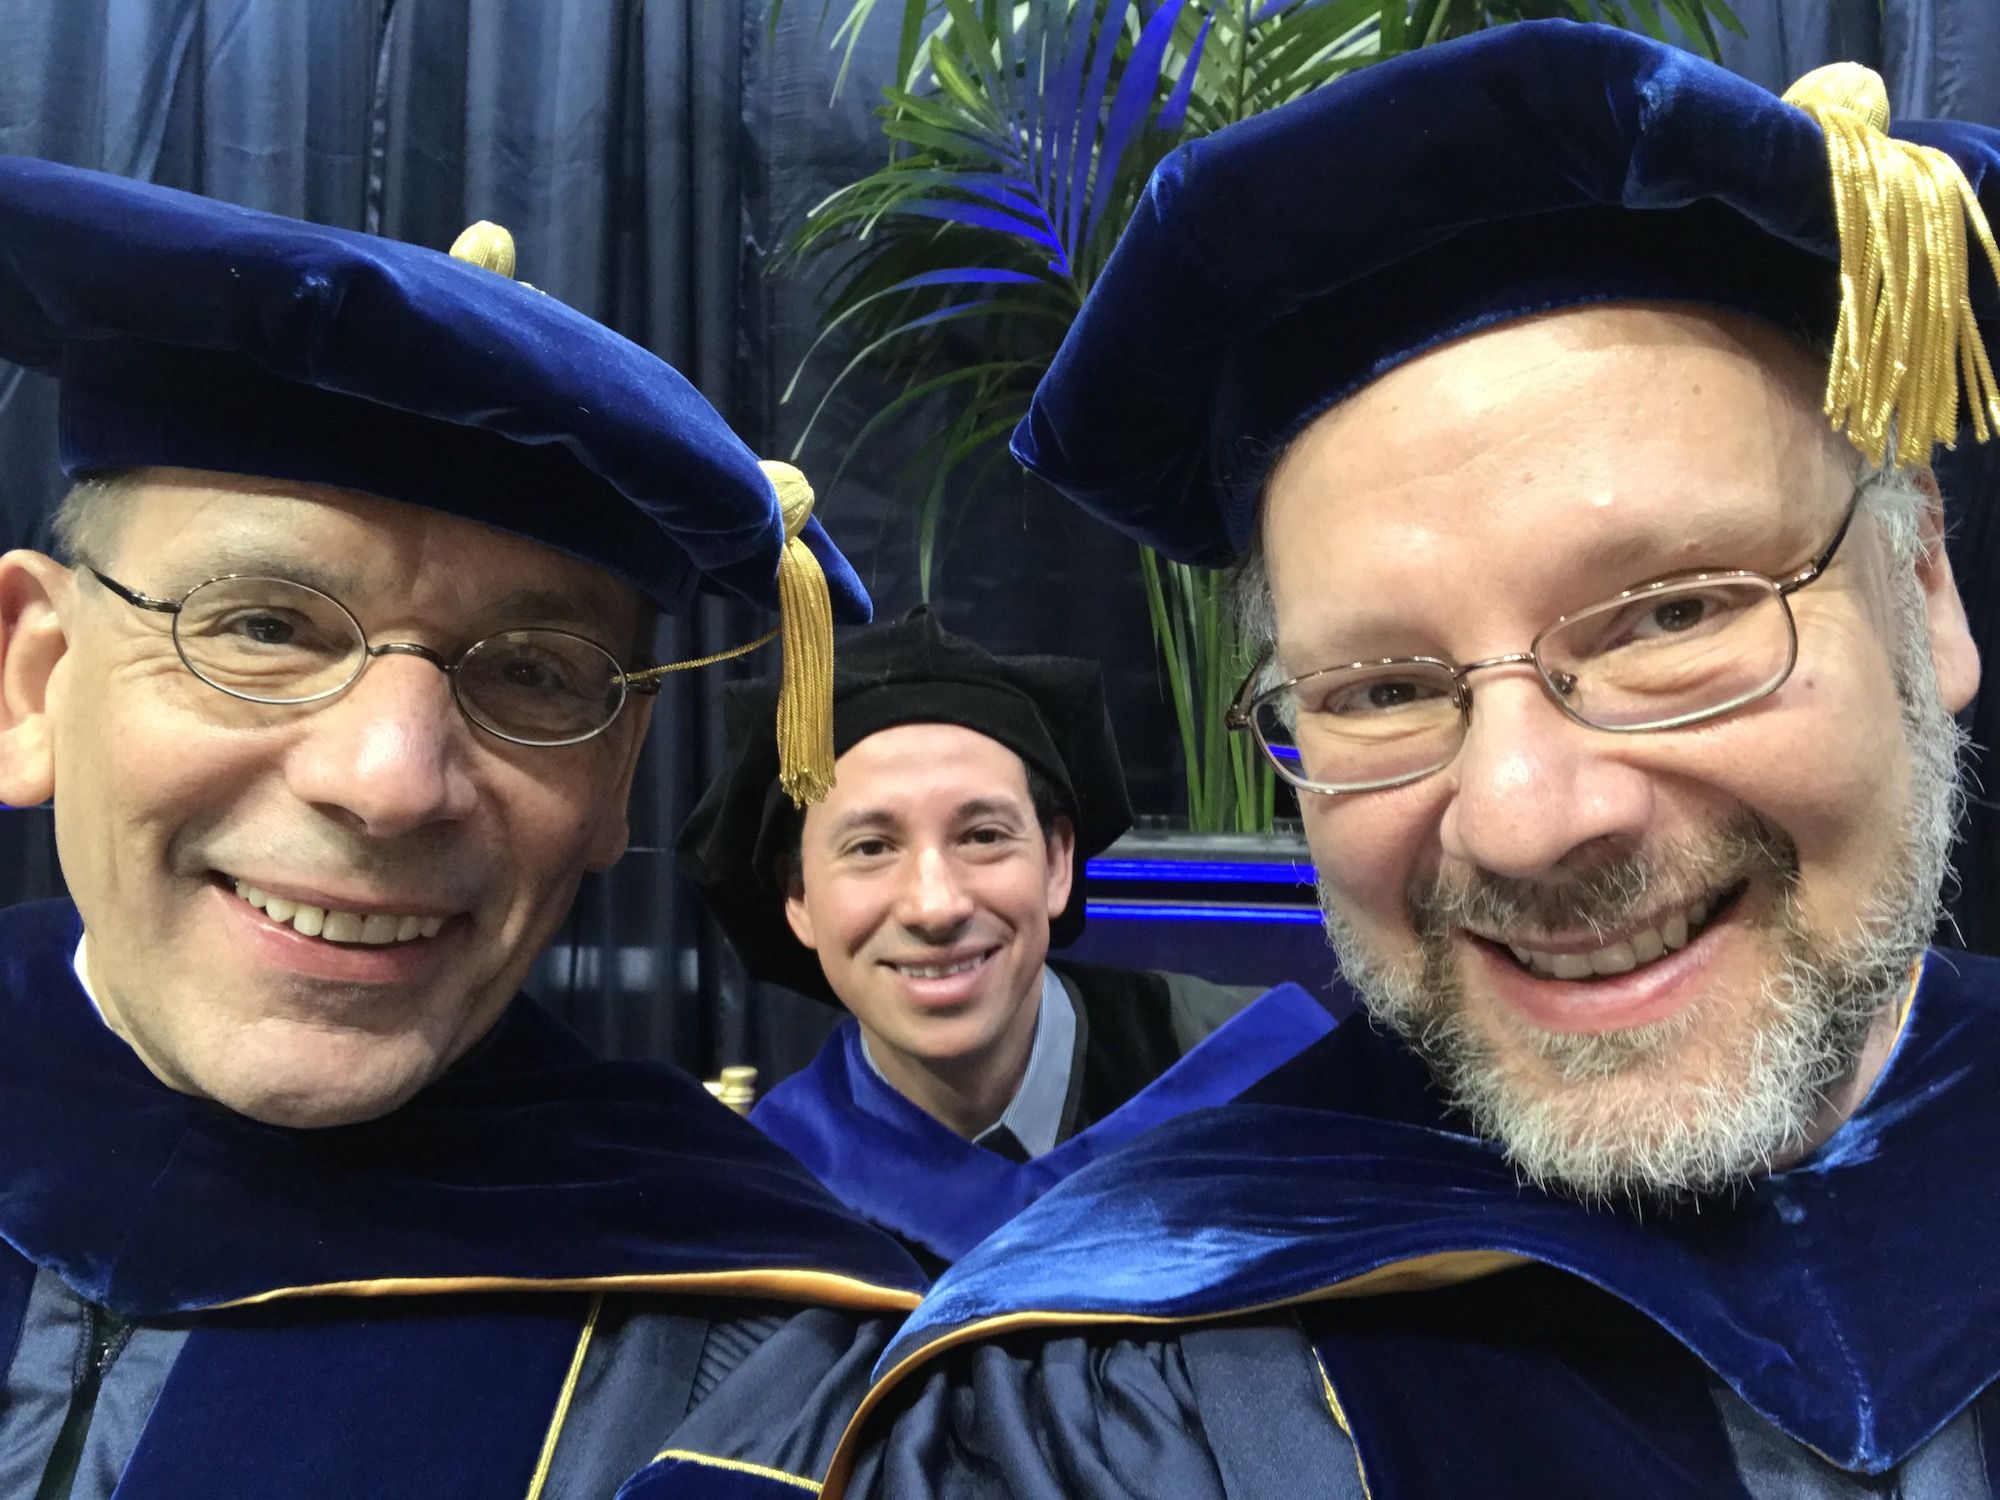
\includegraphics[width=0.45\textwidth]{faculty/graduation}
\end{center}

\restoregeometry
\newpage

